\documentclass{beamer}

\mode<presentation> {

%\usetheme{default}
%\usetheme{AnnArbor}
%\usetheme{Antibes}
%\usetheme{Bergen}
%\usetheme{Berkeley}
%\usetheme{Berlin}
%\usetheme{Boadilla}
%\usetheme{CambridgeUS}
%\usetheme{Copenhagen}
%\usetheme{Darmstadt}
%\usetheme{Dresden}
%\usetheme{Frankfurt}
%\usetheme{Goettingen}
%\usetheme{Hannover}
%\usetheme{Ilmenau}
%\usetheme{JuanLesPins}
%\usetheme{Luebeck}
\usetheme{Madrid}
%\usetheme{Malmoe}
%\usetheme{Marburg}
%\usetheme{Montpellier}
%\usetheme{PaloAlto}
%\usetheme{Pittsburgh}
%\usetheme{Rochester}
%\usetheme{Singapore}
%\usetheme{Szeged}
%\usetheme{Warsaw}

%\usecolortheme{albatross}
%\usecolortheme{beaver}
%\usecolortheme{beetle}
%\usecolortheme{crane}
%\usecolortheme{dolphin}
%\usecolortheme{dove}
%\usecolortheme{fly}
%\usecolortheme{lily}
%\usecolortheme{orchid}
%\usecolortheme{rose}
%\usecolortheme{seagull}
%\usecolortheme{seahorse}
%\usecolortheme{whale}
%\usecolortheme{wolverine}

%\setbeamertemplate{footline} % To remove the footer line in all slides uncomment this line
%\setbeamertemplate{footline}[page number] % To replace the footer line in all slides with a simple slide count uncomment this line

\setbeamertemplate{navigation symbols}{} % To remove the navigation symbols from the bottom of all slides uncomment this line
}

\usepackage{graphicx} % Allows including images
\usepackage{booktabs} % Allows the use of \toprule, \midrule and \bottomrule in tables
\usepackage{listings} % Allows the use of \toprule, \midrule and \bottomrule in tables
\lstset{showstringspaces=false}
%----------------------------------------------------------------------------------------
%	TITLE PAGE
%----------------------------------------------------------------------------------------

\title[Extending Python]{Extending Python}

\author{Francisco Fernandez Castano} % Your name
\institute[@fcofdezc] % Your institution as it will appear on the bottom of every slide, may be shorthand to save space
{
graphenedb.com \\ % Your institution for the title page
\medskip
\textit{francisco.fernandez.castano@gmail.com}
\textit{@fcofdezc}
}
\date{\today} % Date, can be changed to a custom date

\begin{document}

\begin{frame}
\titlepage % Print the title page as the first slide
\begin{center}
http://kcy.me/1gkzu
\end{center}
\end{frame}

\begin{frame}
  \frametitle{Overview}
  \tableofcontents
\end{frame}

\lstset{language=python,
  basicstyle=\ttfamily,
  keywordstyle=\color{blue}\ttfamily,
  stringstyle=\color{red}\ttfamily,
  commentstyle=\color{green}\ttfamily,
  morecomment=[l][\color{magenta}]{\#}
}

\defverbatim[colored]\lstcffitripas{
\begin{lstlisting}[language=c,basicstyle=\footnotesize\ttfamily,keywordstyle=\color{red}]
static PyObject *
b_load_library(PyObject *self, PyObject *args)
{
    void *handle;
    DynLibObject *dlobj;

    if ((flags & (RTLD_NOW | RTLD_LAZY)) == 0)
        flags |= RTLD_NOW;

    printable_filename = filename_or_null ? filename_or_null : "<None>";
    handle = dlopen(filename_or_null, flags);

    dlobj = PyObject_New(DynLibObject, &dl_type);
    dlobj->dl_handle = handle;
    dlobj->dl_name = strdup(printable_filename);
    return (PyObject *)dlobj;
}
\end{lstlisting}
}



\defverbatim[colored]\lstman{
\begin{lstlisting}[language=bash,basicstyle=\ttfamily,keywordstyle=\color{red}]
NAME
dlopen--load and link a dynamic library or bundle

SYNOPSIS
#include <dlfcn.h>

void*
dlopen(const char* path, int mode);
\end{lstlisting}
}

\defverbatim[colored]\lstdlopen{
\begin{lstlisting}[language=c,basicstyle=\ttfamily,keywordstyle=\color{red}]
handle = dlopen(pathname, dlopenflags);

if (handle == NULL) {
    const char *error = dlerror();
    if (error == NULL)
        error = "unknown dlopen() error";
    PyErr_SetString(PyExc_ImportError, error);
    return NULL;
}
if (fp != NULL && nhandles < 128)
    handles[nhandles++].handle = handle;
p = (dl_funcptr) dlsym(handle, funcname);

return p;
\end{lstlisting}
}

\defverbatim[colored]\lsterror{
\begin{lstlisting}[language=c,basicstyle=\ttfamily,keywordstyle=\color{red}]
if (err < 0) {
  PyErr_SetString(PyExc_Exception, "Err");
  return NULL;
}
\end{lstlisting}
}

\defverbatim[colored]\lstpythree{
\begin{lstlisting}[language=c,basicstyle=\ttfamily,keywordstyle=\color{red}]
static struct PyModuleDef examplemodule = {
  PyModuleDef_HEAD_INIT,
  "newton",
  "newton module doc string",
  -1,
  module_functions,
  NULL,
  NULL,
  NULL,
  NULL};
\end{lstlisting}
}

\defverbatim[colored]\lstpythreetwo{
\begin{lstlisting}[language=c,basicstyle=\ttfamily,keywordstyle=\color{red}]
PyMODINIT_FUNC
PyInit_sum(void)
{
PyModule_Create(&examplemodule);
}
\end{lstlisting}
}

\defverbatim[colored]\lstfibc{
\begin{lstlisting}[language=c,basicstyle=\ttfamily,keywordstyle=\color{red}]
int fib(int n){
  if (n < 2)
      return n;
  else
      return fib(n - 1) + fib(n - 2);
}
\end{lstlisting}
}

\defverbatim[colored]\lstfibpy{
\begin{lstlisting}[language=python,basicstyle=\ttfamily,keywordstyle=\color{red}]
import ctypes
lib_fib = ctypes.CDLL("libfib.so")

def ctypes_fib(n):
    return lib_fib.fib(ctypes.c_int(n))

def py_fib(n):
    if n < 2:
       return n
    else:
       return py_fib(n-1) + py_fib(n-2)
\end{lstlisting}
}


\defverbatim[colored]\lstfibres{
\begin{lstlisting}[language=python,basicstyle=\ttfamily,keywordstyle=\color{red}]
In [3]: %timeit fib.ctypes_fib(20)
10000 loops, best of 3: 63.8 micro s per loop

In [4]: %timeit fib.py_fib(20)
100 loops, best of 3: 3.62 ms per loop
\end{lstlisting}
}

\defverbatim[colored]\lstfortran{
\begin{lstlisting}[language=fortran,basicstyle=\ttfamily,keywordstyle=\color{red}]
real(dp) function mean_dp(x, mask)
    implicit none
    real(dp),intent(in) :: x(:)
    logical,intent(in),optional :: mask(:)
    if(present(mask)) then
       mean_dp = sum(x, mask=mask)/size(x)
    else
       mean_dp = sum(x)/size(x)
    end if
end function mean_dp
\end{lstlisting}
}

\defverbatim[colored]\lstforcmd{
\begin{lstlisting}[language=bash,basicstyle=\footnotesize\ttfamily,keywordstyle=\color{red}]
  gfortran -fPIC -shared statistic.f90 -o lib_statistics.so
\end{lstlisting}
}


\defverbatim[colored]\lstforsym{
\begin{lstlisting}[language=fortran,basicstyle=\footnotesize\ttfamily,keywordstyle=\color{red}]
bin git:(master) -> nm -g lib_statistics.so
001eab T ___lib_statistics_MOD_clipped_mean_dp
000afc T ___lib_statistics_MOD_clipped_mean_sp
00306c T ___lib_statistics_MOD_mean_dp
001c55 T ___lib_statistics_MOD_mean_sp
002db0 T ___lib_statistics_MOD_median_dp
0019b0 T ___lib_statistics_MOD_median_sp
002544 T ___lib_statistics_MOD_quantile_dp
00115a T ___lib_statistics_MOD_quantile_sp
002299 T ___lib_statistics_MOD_variance_dp
000ec3 T ___lib_statistics_MOD_variance_sp
U __gfortran_arandom_r4
U __gfortran_arandom_r8
U __gfortran_os_error
U __gfortran_pack
U __gfortran_pow_i4_i4
U __gfortran_runtime_error
U __gfortran_runtime_error_at
U __gfortran_st_write
U __gfortran_st_write_done
U __gfortran_stop_string
\end{lstlisting}
}

\defverbatim[colored]\lstforpy{
\begin{lstlisting}[language=python,basicstyle=\footnotesize\ttfamily,keywordstyle=\color{red}]
from ctypes import *

# Statistics fortran lib
st_lib = CDLL('lib_statistics.so')

mean = st_lib.__lib_statistics_MOD_mean_dp
mean.argtypes = [POINTER(c_float*2)]
mean.restype = c_float

vals = (c_float*2)(2.0, 3.0)

print mean(vals)
\end{lstlisting}
}


\defverbatim[colored]\lstctypesdl{
\begin{lstlisting}[language=c,basicstyle=\footnotesize\ttfamily,keywordstyle=\color{red}]
static PyObject *py_dl_open(PyObject *self, PyObject *args)
{
  char *name;
  void * handle;
  #ifdef RTLD_LOCAL
    int mode = RTLD_NOW | RTLD_LOCAL;
  #else
    /* cygwin doesn't define RTLD_LOCAL */
    int mode = RTLD_NOW;
  #endif
  if (!PyArg_ParseTuple(args, "z|i:dlopen", &name, &mode))
     return NULL;
  mode |= RTLD_NOW;
  handle = ctypes_dlopen(name, mode);
  .
  return PyLong_FromVoidPtr(handle);
}
\end{lstlisting}
}


\defverbatim[colored]\lstcffione{
\begin{lstlisting}[language=python,basicstyle=\footnotesize\ttfamily,keywordstyle=\color{red}]
from cffi import FFI

ffi = FFI()
ffi.cdef("""int printf(const char *format, ...);""")
C = ffi.dlopen(None)
arg = ffi.new("char[]", "world")
C.printf("hi there, %s!\n", arg)
\end{lstlisting}
}

\defverbatim[colored]\lstcffitwo{
\begin{lstlisting}[language=python,basicstyle=\footnotesize\ttfamily,keywordstyle=\color{red}]
from cffi import FFI

ffi = FFI()
ffi.cdef("""int fib(int n);""")
libfib = ffi.dlopen('libfib.so')
libfib.fib(10)
\end{lstlisting}
}

\defverbatim[colored]\lstcffithree{
\begin{lstlisting}[language=python,basicstyle=\footnotesize\ttfamily,keywordstyle=\color{red}]
import cffi
ffi = cffi.FFI()

ffi.cdef("""int fib(int n);""")

ffi.set_source("_fib", r'''
int fib(int n){
if ( n < 2 )
return n;
else
return fib(n-1) + fib(n-2);
}''')

if __name__ == '__main__':
  ffi.compile()
\end{lstlisting}
}

\defverbatim[colored]\lstcffiusage{
\begin{lstlisting}[language=python,basicstyle=\footnotesize\ttfamily,keywordstyle=\color{red}]
  from _fib import fib
  print(fib(10))
\end{lstlisting}
}

\defverbatim[colored]\lstcffifour{
\begin{lstlisting}[language=python,basicstyle=\footnotesize\ttfamily,keywordstyle=\color{red}]
  from _fib import fib
  print(fib("asdasd"))
\end{lstlisting}
}

\defverbatim[colored]\lstcffiboom{
\begin{lstlisting}[language=python,basicstyle=\footnotesize\ttfamily,keywordstyle=\color{red}]
Traceback (most recent call last):
File "fib.py", line 16, in <module>
print lib.fib("asd")
TypeError: an integer is required
\end{lstlisting}
}

\defverbatim[colored]\lstcffistruct{
\begin{lstlisting}[language=python,basicstyle=\footnotesize\ttfamily,keywordstyle=\color{red}]
from cffi import FFI
ffi = FFI()
ffi.cdef("""typedef struct { float x, y; } point;""")
point = ffi.new("point *")
point.x = 2.0
point.y = 3.0
\end{lstlisting}
}





\defverbatim[colored]\lstsetup{
\begin{lstlisting}[language=python,basicstyle=\ttfamily,keywordstyle=\color{red}]
from distutils.core import setup, Extension

setup(name='fosdem',
      version=1.0,
      ext_modules=[
        Extension('newton', ['newton.c'])])
\end{lstlisting}
}

\defverbatim[colored]\lstflowconverted{
\begin{lstlisting}[language=python,basicstyle=\ttfamily,keywordstyle=\color{red}]
Block(v1):     # input argument
  v2 = mul(Constant(3), v1)
  v3 = add(v2, Constant(2))
\end{lstlisting}
}

\defverbatim[colored]\lstyoung{
  \begin{lstlisting}[language=python,basicstyle=\ttfamily,keywordstyle=\color{red}]
    [elem * 2 for elem in elements]
    balance = (a / b / c) * 4
    'asdadsasd-xxx'.replace('x', 'y').replace('a', 'b')
    foo.bar()
  \end{lstlisting}
}

\defverbatim[colored]\lstsymbols{
  \begin{lstlisting}[language=bash,basicstyle=\ttfamily,keywordstyle=\color{red}]
$ nm -g newton.so
00000000002010a0 B __bss_start
                 w __cxa_finalize@@GLIBC_2.2.5
00000000002010a0 D _edata
00000000002010a8 B _end
0000000000000944 T _fini
                 w __gmon_start__
00000000000006d0 T _init
0000000000000920 T initnewton
                 w _ITM_deregisterTMCloneTable
                 w _ITM_registerTMCloneTable
                 w _Jv_RegisterClasses
                 U PyArg_ParseTuple
                 U Py_BuildValue
                 U Py_InitModule4_64
  \end{lstlisting}
}

\defverbatim[colored]\lstctypesstruct{
  \begin{lstlisting}[language=python,basicstyle=\ttfamily,keywordstyle=\color{red}]
from ctypes import *

class POINT(Structure):
    _fields_ = [("x", c_int), ("y", c_int)]

class RECT(Structure):
    _fields_ = [("upperleft", POINT),
                ("lowerright", POINT)]
  \end{lstlisting}
}



\defverbatim[colored]\lstnative{
  \begin{lstlisting}[language=c,basicstyle=\footnotesize\ttfamily,keywordstyle=\color{red}]
#include "Python.h"

static PyObject *
newton(PyObject *self, PyObject *args)
{
    float guess;
    float x;

    if (!PyArg_ParseTuple(args, "ff", &guess, &x))
        return NULL;

    while (fabs(powf(guess, 2) - x) > 0.01)
    {
        guess = ((x / guess) + guess) / 2;
    }

    return Py_BuildValue("f", guess);
}
  \end{lstlisting}
}

\defverbatim[colored]\lstnativen{
  \begin{lstlisting}[language=c,basicstyle=\footnotesize\ttfamily,keywordstyle=\color{red}]

static PyMethodDef
module_functions[] = {
    {"newton", newton, METH_VARARGS, "Newton method."},
    {NULL}
};


PyMODINIT_FUNC
initnewton(void)
{
    Py_InitModule3("newton", module_functions, "Newton");
}
  \end{lstlisting}
}

\defverbatim[colored]\lststatic{
\begin{lstlisting}[language=bash,basicstyle=\ttfamily,keywordstyle=\color{red}]
$ ar tv libdemo.a
rw-r--r-- 501/20 40 Jul 19 22:34 2014 __.SYMDEF
rw-r--r-- 501/20 2352 Jul 19 22:33 2014 a.o
rw-r--r-- 501/20 2352 Jul 19 22:33 2014 b.o
\end{lstlisting}
}

\defverbatim[colored]\lstnewtonout{
\begin{lstlisting}[language=python,basicstyle=\ttfamily,keywordstyle=\color{red}]
Python 2.7.5 (default, Nov  3 2014, 14:26:24)
[GCC 4.8.3 20140911 (Red Hat 4.8.3-7)] on linux2
>>> import newton
>>> newton.newton(1, 2)
1.4166667461395264
>>>
\end{lstlisting}
}


\section{Motivations}

\begin{frame}{Caution}
    \begin{itemize}
    \item Huge topic
    \item \textit{Toy} examples
    \item Unix \^ CPython centric
    \end{itemize}
\end{frame}

\begin{frame}{Motivation}
  Why write in C?
\end{frame}

\begin{frame}{Motivation}
  \begin{itemize}
  \item \textbf{Speed}
  \item Using legacy code
  \item Integration
  \end{itemize}
\end{frame}

\begin{frame}{Motivation}
\framesubtitle{Why is Python \textit{slow}?}
  \begin{itemize}
    \item Interpretation overhead
    \item Boxed arithmetic and automatic overflow handling
    \item Dynamic dispatch of operations
    \item Dynamic lookup of methods and attributes
    \item Everything can change on runtime
    \item Extreme introspective and reflective capabilities
  \end{itemize}
\end{frame}

\begin{frame}{Motivation}
  \begin{itemize}
  \item Speed
  \item \textbf{Using legacy code}
  \item Integration
  \end{itemize}
\end{frame}

\begin{frame}{Motivation}
  \begin{itemize}
  \item Speed
  \item Using legacy code
  \item \textbf{Integration}
  \end{itemize}
\end{frame}

\section{Guidelines}

% \begin{frame}{Guidelines}
%   \begin{itemize}
%     \item Static libraries
%     \item Shared libraries
%   \end{itemize}
% \end{frame}


% \begin{frame}{Static libraries}
% \begin{block}{}
%   \lststatic
% \end{block}
% \end{frame}

\begin{frame}{Shared libraries}
  \begin{itemize}
    \item Single copy in memory
    \item Runtime load
  \end{itemize}
\end{frame}

\section{Native extensions}

\begin{frame}{Native extensions}
  C API
\end{frame}

\begin{frame}{Native extensions}
  \textit{Hello world, Newton method}
\end{frame}

\begin{frame}{Native extensions}
    \begin{figure}
      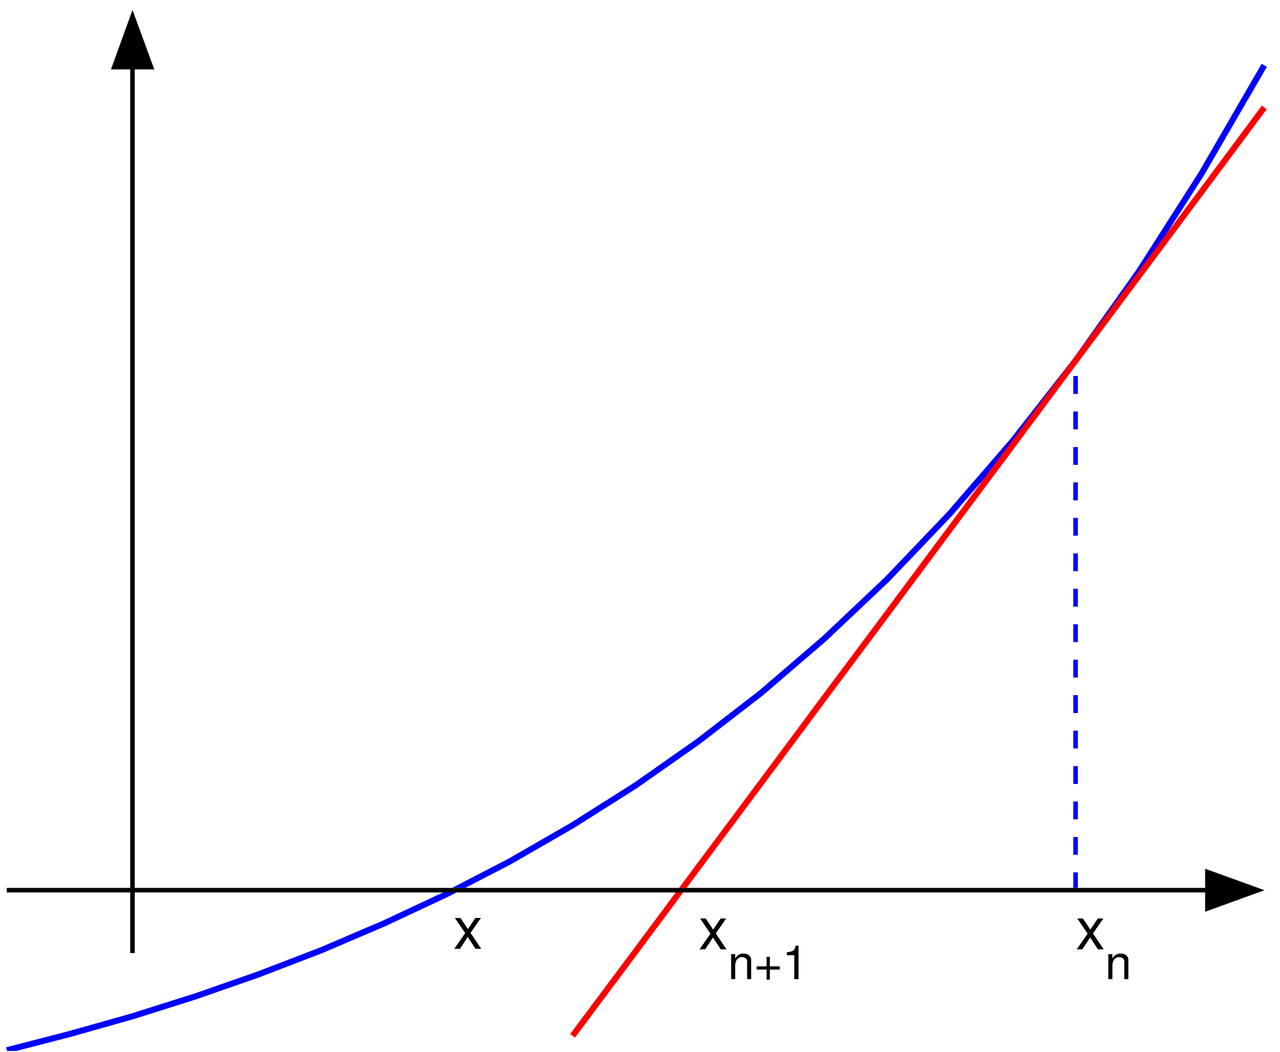
\includegraphics[width=0.6\linewidth]{newton.png}
    \end{figure}
\end{frame}

\begin{frame}{Native extensions}
\begin{block}{}
  \lstnative
\end{block}
\end{frame}

\begin{frame}{Native extensions}
\begin{block}{}
  \lstnativen
\end{block}
\end{frame}

\begin{frame}{Native extensions}
\begin{block}{}
  \lstsetup
\end{block}
\end{frame}

\begin{frame}{Native extensions}
\begin{block}{}
  \lstnewtonout
\end{block}
\end{frame}

\begin{frame}{How?}
    \begin{figure}
      
\includegraphics[width=0.7\linewidth]{sagan.jpg}
    \end{figure}
\end{frame}


\begin{frame}{Native extensions}
\begin{block}{}
  \lstman
\end{block}
\end{frame}

\begin{frame}{Native extensions}
\begin{block}{}
  \lstsymbols
\end{block}
\end{frame}

\begin{frame}{Native extensions}
\begin{block}{cpython/Python/dynload\_shlib.c}
  \lstdlopen
\end{block}
\end{frame}

\begin{frame}{Native extensions}
  \framesubtitle{Memory management}
  \begin{itemize}
  \item Manual memory management
  \item Python GC - RC
  \item Cycle detector
  \item Py\_INCREF(x) Py\_DECREF(x)
  \end{itemize}
\end{frame}

\begin{frame}{Native extensions}
  \framesubtitle{Error management}
  \begin{itemize}
  \item Return NULL as a convention
  \item Register exceptions
  \end{itemize}
\end{frame}

\begin{frame}{Native extensions}
  \framesubtitle{Error management}
  \begin{block}{}
    \lsterror
  \end{block}
\end{frame}


\begin{frame}{Native extensions}
  \framesubtitle{Python 3 differences}
  \begin{block}{}
    \lstpythree
  \end{block}
\end{frame}

\begin{frame}{Native extensions}
  \framesubtitle{Python 3 differences}
  \begin{block}{}
    \lstpythreetwo
  \end{block}
\end{frame}

\section{CTypes}
\begin{frame}{CTypes}
  \begin{itemize}
   \item Advanced FFI for Python
   \item Allows call functions from Shared libs
   \item Create, access, manipulate C data types
  \end{itemize}
\end{frame}

\begin{frame}{CTypes}
  \framesubtitle{Types correspondence}
    \begin{figure}
      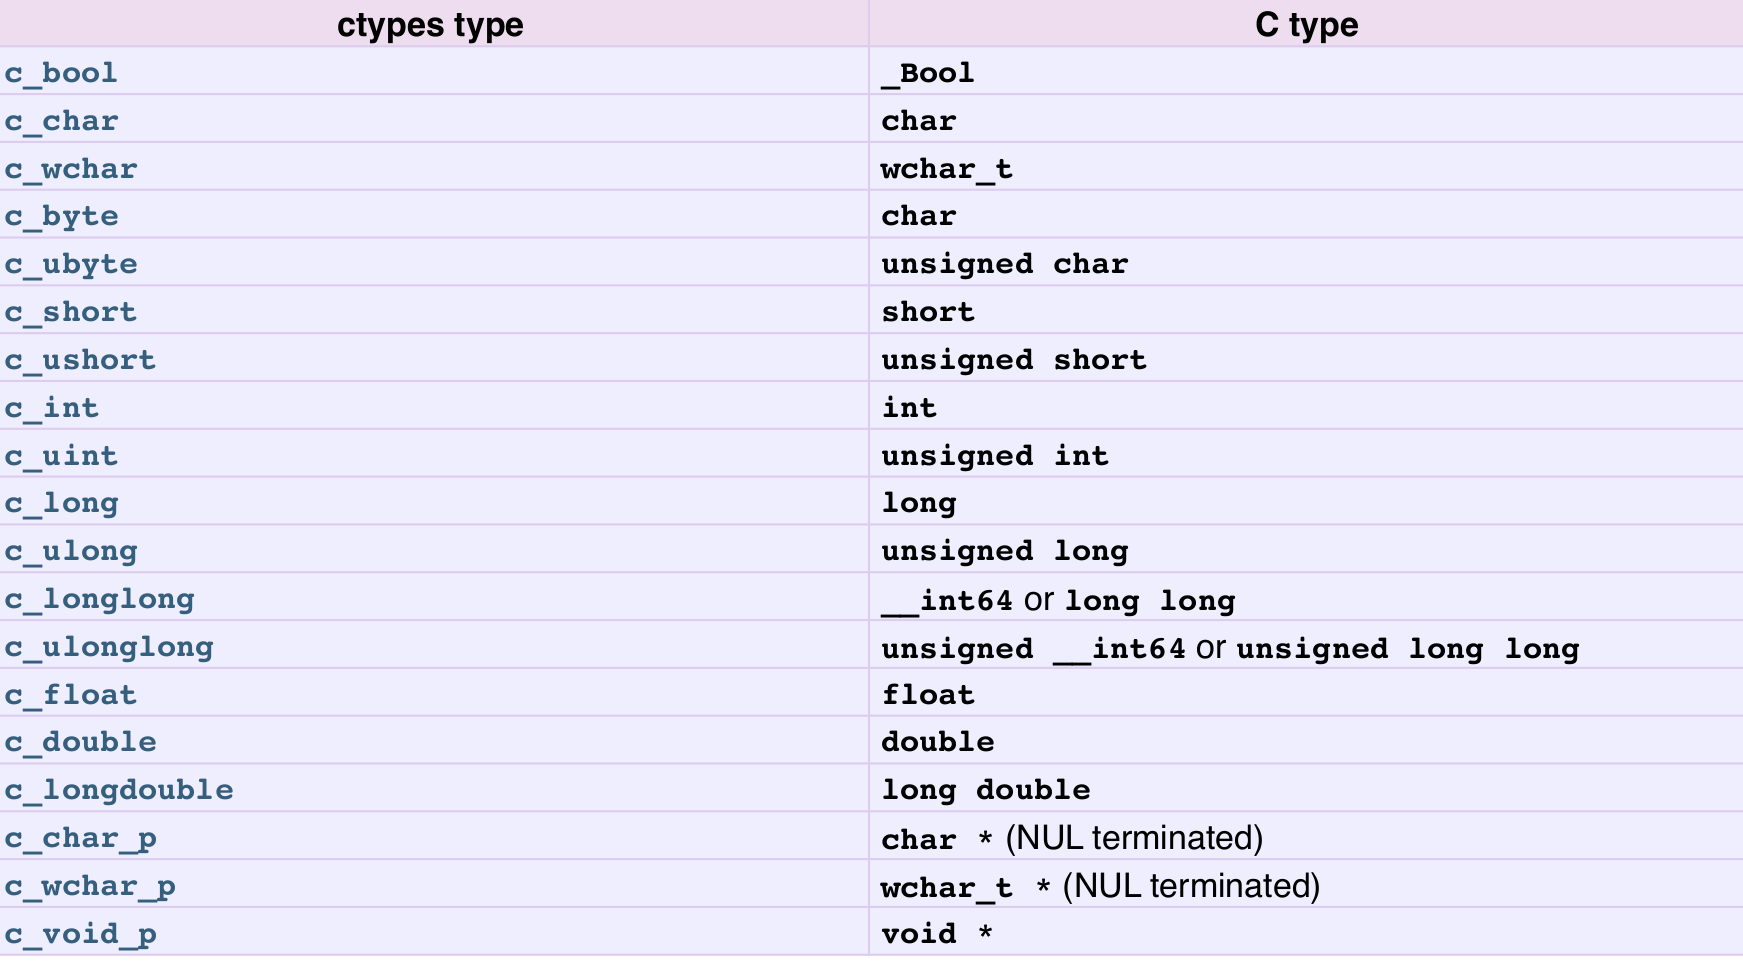
\includegraphics[width=0.9\linewidth]{ctypes.png}
    \end{figure}
\end{frame}

\begin{frame}{CTypes}
  \framesubtitle{Structs}
  \begin{block}{}
  \lstctypesstruct
  \end{block}
\end{frame}


\begin{frame}{CTypes}
  \framesubtitle{Example}
  \begin{itemize}
    \item Implemented fibonacci as c function
    \item Map as Python code
    \item Measure differences between Python and C
  \end{itemize}
\end{frame}

\begin{frame}{CTypes}
  \begin{block}{}
  \lstfibc
  \end{block}
\end{frame}

\begin{frame}{CTypes}
  \begin{block}{}
  \lstfibpy
  \end{block}
\end{frame}

\begin{frame}{CTypes}
  \begin{block}{}
  \lstfibres
  \end{block}
\end{frame}


\begin{frame}{CTypes}
  \framesubtitle{Fortran example}
  \begin{itemize}
    \item Use of existing fortran code
    \item Take random code at github
    \item https://github.com/astrofrog/fortranlib
    \item Wrap using ctypes
  \end{itemize}
\end{frame}

\begin{frame}{CTypes}
  \framesubtitle{Fortran example}
  \begin{block}{}
    \lstfortran
  \end{block}
\end{frame}

\begin{frame}{CTypes}
  \framesubtitle{Fortran example}
  \begin{block}{}
  \lstforcmd
  \end{block}
\end{frame}


\begin{frame}{CTypes}
  \framesubtitle{Fortran example}
  \begin{block}{}
  \lstforsym
  \end{block}
\end{frame}

\begin{frame}{CTypes}
  \framesubtitle{Fortran example}
  \begin{block}{}
  \lstforpy
  \end{block}
\end{frame}

\begin{frame}{CTypes}
  \framesubtitle{CTypes source}
  \begin{block}{cpython/Modules/\_ctypes/callproc.c}
  \lstctypesdl
  \end{block}
\end{frame}

\section{CFFI}

\begin{frame}{CFFI}
  \begin{itemize}
  \item Advanced FFI for Python
  \item Allows call functions from Shared libs
  \item Create, access, manipulate C data types
  \item Both API and ABI access
  \end{itemize}
\end{frame}

\begin{frame}{CFFI}
  Mostly the same as CTypes
\end{frame}

\begin{frame}{CFFI}
  Recommended way to extend PyPy
\end{frame}

\begin{frame}{CFFI}
  \framesubtitle{ABI}
  \begin{block}{}
    \lstcffione
  \end{block}
\end{frame}

\begin{frame}{CFFI}
  \framesubtitle{ABI- Fibonacci}
  \begin{block}{}
    \lstcffitwo
  \end{block}
\end{frame}

\begin{frame}{CFFI}
  \framesubtitle{API Level}
  \begin{block}{}
    \lstcffithree
  \end{block}
\end{frame}

\begin{frame}{CFFI}
  \framesubtitle{API Level}
  \begin{block}{}
    \lstcffiusage
  \end{block}
\end{frame}

\begin{frame}{CFFI}
  \framesubtitle{API Level}
  \begin{block}{}
    \lstcffifour
  \end{block}
\end{frame}

\begin{frame}{CFFI}
  \framesubtitle{API Level}
  \begin{block}{}
    \lstcffiboom
  \end{block}
\end{frame}

\begin{frame}{CFFI}
  \framesubtitle{API Level}
  \begin{block}{}
    \lstcffistruct
  \end{block}
\end{frame}

\begin{frame}{CFFI}
  \framesubtitle{Internals}
  \begin{block}{cffi/c/\_cffi\_backend.c}
    \lstcffitripas
  \end{block}
\end{frame}

\section{Conclusions}

\begin{frame}{Conclusions}
  \begin{itemize}
    \item Three different ways
    \item Same principles
    \item Less portable - More portable
    \item Harder - Easier
  \end{itemize}
\end{frame}

\begin{frame}{}
  \begin{figure}
      
\includegraphics[width=0.9\linewidth]{questions.jpg}
  \end{figure}
\end{frame}


\end{document}
